\section{قانون یادگیری تقویتی}
    انعطاف‌پذیری وابسته به زمان ضربه تعدیل‌شده با پاداش 
    ($R-STDP$)\footnote{\lr{Reward-Modulated Spike-Timing-Dependent Plasticity}}
    به عنوان یک مدل پیچیده برای درک چگونگی تکامل ارتباطات سیناپسی بر اساس زمان‌بندی ضربه های عصبی و تأثیر سیگنال‌های پاداش عمل می‌کند. این مدل، که شامل تعدیل کننده های عصبی مانند دوپامین است، قدرت سیناپسی را برای ترویج رفتارهایی که منجر به پاداش می شود، تنظیم می کند. در اینجا، پیاده‌سازی 
    $R-STDP$ 
    را بررسی می‌کنیم که این پویایی‌ها را در یک چارچوب محاسباتی ادغام می‌کند و مطالعه مکانیسم‌های یادگیری را که زیربنای فرآیندهای یادگیری مبتنی بر پاداش است، تسهیل می‌کند.

    مدل 
    $R-STDP$ 
    که در اینجا پیاده سازی کرده ام، مکانیسم کلاسیک 
    $STDP$ 
    را با ترکیب اثرات دوپامین، که به عنوان یک سیگنال بازخورد برای تقویت یا مجازات اعمال عمل می کند، گسترش می دهد. این مدل برای رسیدگی به پیچیدگی‌های انعطاف‌پذیری سیناپسی تحت تأثیر زمان‌ ضربه ها و حضور سیگنال‌های پاداش، نوشته شده است.
    \begin{itemize}
        \item \textbf{ردیابی های سیناپسی و دوپامین:} 
        این مدل از اثر 
        (ردپا)
        های پیش سیناپسی و پس سیناپسی استفاده می کند که در طول زمان با ثابت های 
        $\tau_{pre}$ 
        و 
        $tau_{post}$ 
        کاهش می یابند. این ردپا ها زمان ضربه ها را ثبت می کنند و به عنوان یک متغیر اصلی برای محاسبه تغییرات سیناپسی عمل می کنند.
        \item \textbf{به‌روزرسانی‌ وزن ها با دوپامین:} 
        به‌روزرسانی‌های اثربخشی سیناپسی به تعامل بین آثار ضربه و سطوح دوپامین بستگی دارد، که به معنای این است که رفتار ها منجر به افزایش ضربه شده است یا خیر. این مدل به صورت پویا وزن ها را بر اساس اینکه آیا رفتار ها با نتایج مثبت 
        (دوپامین مثبت) 
        یا نتایج منفی 
        (دوپامین منفی) 
        مرتبط است، تنظیم می کند.
        \item \textbf{پاسخ‌های متفاوت دوپامین:} 
        این مدل بین سیگنال‌های دوپامین مثبت و منفی، تمایز قائل می‌شود که وزن‌های سیناپسی را بر این اساس تعدیل می‌کنند. این تنظیم دوگانه به مدل اجازه می دهد تا نقاط قوت سیناپسی را بر اساس نتایج خاص اقدامات تنظیم کند.
    \end{itemize}
    پاداش دادن به وزن ها نیز میتواند با روش های مختلفی انجام پذیرد. به عنوان مثال، ورودی نوع 
    $A$ 
    به شبکه ورودی داده می شود و انتظار داریم نورون خروجی شماره ۱ آن را تشخیص دهد. این تشخیص دادن را می توان به دو صورت در نظر گرفت. یک روش آن که نورونی که زودتر ضربه می زند، این تشخیص را انجام داده است، روش دیگر آنکه نورونی که در پنجره زمانی ورودی دادن بیشترین نرخ ضربه را داشته است، آن را تشخیص داده است. بسته به اینکه کدام روش انتخاب شود، به وزن های هر یک از نورون ها میتوانیم دوپامین ها را اعمال کنیم. من بدلیل آنکه ورودی ها نیز به صورت نرخ ضربه زدن کدگذاری شده بودند، از روش دوم برای تشخیص دادن نیز استفاده کردم.

    \subsection{آزمایش ها}
        \paragraph*{شباهت کسینوسی:}
                \textbf{ دقت شود که نمودار شباهت کسینوسی در تمام شکل ها آمده است.}

        حال به سراع آزمایش کردن مدلمان با ورودی و پارامتر های مختلف می رویم. اولین آزمایشی که مطابق معمول انجام میدهیم، ورودی دادن اندازه های مختلف ورودی است.
        \subsubsection*{تاثیر اندازه}
        اولین ورودی، ۲ الگوی ورودی از جنس یک آرایه از اعداد است. همانطور که در شکل 
        \ref{fig:part3-rstdp-small-array}
        نیز مشاهده می شود، مدل به خوبی توانسته است الگو های ورودی را یاد بگیرد.
        ورودی در این مدل، شامل دو آرایه تصادفی است که مقادیر یکی، دو برابر دیگری ست. مقادیر 
        \begin{figure}[!ht]
            \centering
            \captionsetup{width=.9\linewidth}
            \includegraphics[width=0.9\textwidth]{plots/part3-rstdp-small-array.pdf} 
            \caption{همانطور که در شکل مشاهده میکنیم، مدل پس از حدود ۵۰۰ مرحله توانسته است الگو های ورودی را یاد بگیرد. با گذشتن مراحل بیشتر نیز، نورون ها ورودی ها را بیشتر یاد گرفته به طوری که فعالیت کلی آن ها در طول بازه ورودی خود، بیشتر می شود. 
            همانطور که هر نورون در لایه خروجی یاد می‌گیرد که به ویژگی‌های خاص مرتبط با یک کلاس خاص به شدت پاسخ دهد، بردارهای وزن آن‌ها از هم جدا می‌شوند. این واگرایی منجر به کاهش شباهت کسینوسی می‌شود، زیرا بردارهای وزنی با تطتبیق خود برای تشخیص ویژگی‌های متمایز کلاس‌های مختلف، موازی‌تر می‌شوند. }
            \label{fig:part3-rstdp-small-array}
        \end{figure}
        
        حال دو الگوی 
        \ref{fig:part3-pattern1}
        و 
        \ref{fig:part3-pattern2} 
        را به عنوان ورودی به نورون ها ورودی میدهیم تا مشاهده کنیم که آیا شبکه از عهده یادگرفتن دو الگوی ساده برمی آید یا خیر.
        \begin{figure}[!ht]
            \centering
            \captionsetup{width=.9\linewidth}
            \begin{subfigure}[b]{0.35\textwidth}
                \centering
                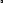
\includegraphics[width=\textwidth]{images/pattern1.png}
                \caption{الگوی اول}
                \label{fig:part3-pattern1}
            \end{subfigure}
            \hfill
            \begin{subfigure}[b]{0.35\textwidth}
                \centering
                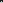
\includegraphics[width=\textwidth]{images/pattern2.png}
                \caption{الگوی دوم}
                \label{fig:part3-pattern2}
            \end{subfigure}
            \caption{دو تصویر به عنوان محرک}
            \label{fig:part3-patterns}
        \end{figure}
        همانطور که از شکل
        \ref{fig:part3-rstdp-small-patterns} 
        نیز بر می آید، نورون ها در یادگیری الگو های ذکر شده موفق بوده اند.

        \begin{figure}[!ht]
            \centering
            \captionsetup{width=.9\linewidth}
            \includegraphics[width=0.9\textwidth]{plots/part3-rstdp-small-patterns.pdf} 
            \caption{قانون یادگیری 
            $RSTDP$ برای دو الگوی ساده. مطابق نمودار بالا دریافت می شود که نورون ها با استفاده از قانون یادگیری 
            $RSTDP$ 
            توانسته اند الگو های 
            \ref{fig:part3-pattern1}
            و 
            \ref{fig:part3-pattern2} 
            را به خوبی یاد بگیرند. به طوری که این یادگیری تا ۵۰۰ مرحله یا به عبارتی با ۳ بار ورودی دادن هر الگو، انجام شده است که نکته قابل توجهی است. تا مرحله ۱۵۰۰ ام شبیه سازی نیز این یادگیری عمیق تر شده و نورون ها  فقط در زمانی که الگوی خود را میبینند ضربه می زنند.
            }
            \label{fig:part3-rstdp-small-patterns}
        \end{figure}
        حال ورودی ها را به طوری که در صورت پروژه گفته شده بود به شبکه میدهیم، یعنی بعضی نورون ها، هر دو الگو را به عنوان ورودی دریافت میکنند.(نورون های سبز در شکل
        \ref{fig:part3-input-overlap})

        \begin{figure}[!ht]
            \centering
            \captionsetup{width=.9\linewidth}
            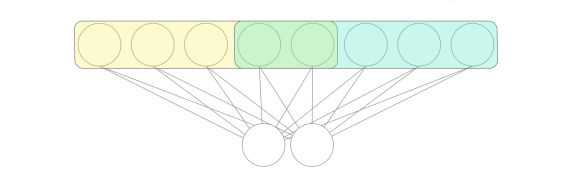
\includegraphics[width=0.9\textwidth]{images/input-overlap.png} 
            \caption{نورون هایی که با رنگ سبز مشخص شده اند، هر دو الگو را به عنوان ورودی دریافت میکنند.
            }
            \label{fig:part3-input-overlap}
        \end{figure}

        مطابق شکل 
        \ref{fig:part3-rstdp-small-patterns-overlap}
        مشاهده میکنیم که هم پوشانی نورون های ورودی در دریافت محرک، باعث می شود که شبکه کمی دیرتر الگو ها را یاد بگیرند.
        \begin{figure}[!ht]
            \centering
            \captionsetup{width=.9\linewidth}
            \includegraphics[width=0.9\textwidth]{plots/part3-rstdp-small-patterns-overlap.pdf} 
            \caption{هم پوشانی نورون ها در دریافت ورودی. مطابق نمودار های بالا، اختصاص بعضی نورون ها به دریافت دو نوع الگو، باعث می شود که شبکه کمی دیرتر الگو ها را یاد بگیرد. به طوری که در مقایسه با شکل
            \ref{fig:part3-rstdp-small-patterns}
            یادگیری در ۳۰۰ مرحله بعد انجام شده است. هر چند هر دو مدل در نهایت الگو های ورودی را فراگرفته اند.
            }
            \label{fig:part3-rstdp-small-patterns-overlap}
        \end{figure}
        حتی اگر میزان همپوشانی را به حداکثر برسانیم
        (به طوری که همه محرک ها به همه نورون ها داده شود)
        باز هم شبکه قادر به تشخیص الگو ها خواهد بود.
        (شکل \ref{fig:part3-rstdp-small-patterns-high-overlap})

        \begin{figure}[!ht]
            \centering
            \captionsetup{width=.9\linewidth}
            \includegraphics[width=0.9\textwidth]{plots/part3-rstdp-small-patterns-high-overlap.pdf} 
            \caption{هم پوشانی حداکثری نورون ها در دریافت ورودی. مشاهده میکنیم که حتی با هم پوشانی کامل نیز، شبکه قادر به یادگیری الگو ها می باشد، هر چند بعضی اوقات نورون ها هنگامی که ورودی دیگر را میبینند نیز ضربه میزنند که اینکار با تنظیم پارامتر ها قابل بهبود است و در بخش بعدی به آن می پردازیم.
            }
            \label{fig:part3-rstdp-small-patterns-high-overlap}
        \end{figure}

        حال در نهایت یک قدم فراتر گذاشته، و دو تصویر با اندازه های 
        $10\times 10$ 
        را به عنوان ورودی به مدل میدهیم.
        (تصاویر 
        \ref{fig:part3-input-image1} و
        \ref{fig:part3-input-image2})

        \begin{figure}[htbp]
            \centering
            \captionsetup{width=.9\linewidth}
            \begin{subfigure}[b]{0.35\textwidth}
                \centering
                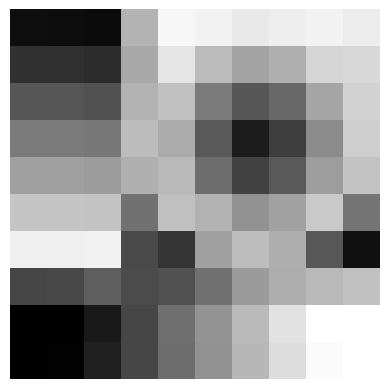
\includegraphics[width=\textwidth]{images/slop-resized.jpg}
                \caption{تصویر اول}
                \label{fig:part3-input-image1}
            \end{subfigure}
            \hfill
            \begin{subfigure}[b]{0.35\textwidth}
                \centering
                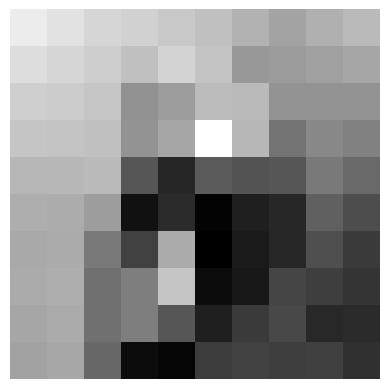
\includegraphics[width=\textwidth]{images/bird-resized.jpg}
                \caption{تصویر دوم}
                \label{fig:part3-input-image2}
            \end{subfigure}
            \caption{یک تصویر به عنوان محرک}
            \label{fig:part3-input-images}
        \end{figure}
        ممکن است انتظار داشته باشیم با زیاد شدن ابعاد ورودی، تشخیص الگوها نیز سخت تر شود، اما شکل 
        \ref{fig:part3-rstdp-images}
        این فرض را رد میکند و مشاهده میکنیم که یادگیری دو الگو به خوبی انجام شده است.

        \begin{figure}[!ht]
            \centering
            \captionsetup{width=.9\linewidth}
            \includegraphics[width=0.9\textwidth]{plots/part3-rstdp-images.pdf} 
            \caption{یادگیری الگوی دو تصویر توسط قانون یادگیری 
            $RSTDP$. مطابق شکل بالا مشاهده میکنیم که با وجود ابعاد بالای الگوی ورودی نیز، یادگیری هنوز به خوبی انجام می شود. نکته قابل توجه دیگری که از این شکل برداشت می شود نیز این است که پس از حدود ۱۵۰۰ مرحله از شبیه سازی، نمودار فعالیت نورون ها ثابت تر می شود، بدان معنا که بین تکرار های ۱۰۰۰ و ۱۵۰۰، فعالیت نورون ها در بعضی لحظه ها 
            $50\%$ 
            ودر بعضی لحظه ها کمتر است اما بعد از تکرار ۱۵۰۰، هر گاه که ورودی مربوط به یک الگو داده می شود، در تمام آن پنجره زمانی، نورون های مربوط ضربه میزنند و پیوسته فعالیت کامل دارند.
            }
            \label{fig:part3-rstdp-images}
        \end{figure}

        مدل نسبت به هم پوشانی نورون ها برای گرفتن ورودی نیز پایدار است و همچنان الگو ها را یاد میگیرد.
        (شکل \ref{fig:part3-rstdp-images-overlap})
        \begin{figure}[!ht]
            \centering
            \captionsetup{width=.9\linewidth}
            \includegraphics[width=0.9\textwidth]{plots/part3-rstdp-images-overlap.pdf} 
            \caption{یادگیری الگوی دو تصویر توسط قانون یادگیری 
            $RSTDP$ با هم پوشانی نورون ها. مطابق شکل ملاحظه میکنیم که هم پوشانی نورون ها در دریافت ورودی نیز نمیتواند از یادگیری الگو ها توسط مدل جلو گیری کند. هرچند این اتفاق کمی دیرتر می افتد که به این دلیل است بعضی نورون ها باید هر دوی الگو ها را یاد بگیرند.
            (توجه کنید که اکنون جمعیت ورودی شامل ۱۵۰ نورون است درحالی که الگو ها ۱۰۰ پیکسل دارند و از آنجا که بیشترین میزان فعالیت نورون ها بعد از یادگیری 
            $50\%$ 
            است، ۷۵ نورون باید ۱۰۰ پیکسل را فراگیرند. به عبارتی دیگر، بعضی نورون ها هر دو الگو را یاد میگیرند.)
            }
            \label{fig:part3-rstdp-images-overlap}
        \end{figure}
        حتی با بیشتر کردن هم پوشانی نیز باز هم مدل می تواند تصاویر را یاد بگیرد.
        (شکل 
        \ref{fig:part3-rstdp-images-high-overlap})
        هر چند نسبت به حالت های قبلی این یادگیری دیرتر اتفاق می افتد، اما با تنظیم پارامتر هایی مانند پنجره زمانی یا دوپامین که در ادامه بررسی می شوند می توان این یادگیری را سریع تر کرد.

        \begin{figure}[!ht]
            \centering
            \captionsetup{width=.9\linewidth}
            \includegraphics[width=0.9\textwidth]{plots/part3-rstdp-images-high-overlap.pdf} 
            \caption{یادگیری الگوی دو تصویر توسط قانون یادگیری 
            $RSTDP$ با هم پوشانی کامل نورون ها.
            همانطور که در نمودار بالا نیز ملاحظه می شود، حتی با هم پوشانی کامل نورون ها نیز دو الگو از یکدیگر تشخیص داده می شوند. نکته ایکه وجود دارد این است که این یادگیری نسبت با حالت های با هم پوشانی کمتر، دیرتر اتفاق می افتد.
            }
            \label{fig:part3-rstdp-images-high-overlap}
        \end{figure}

        
        \clearpage
        \subsubsection*{تاثیر وزن های اولیه}
            در گذشته در شبکه های عصبی کلاسیک، وزن های اولیه ممکن بود تاثیر زیادی در یادگیری شبکه بگذارند. در این بخش ما یادگیری مدلمان را روی دو الگوی ورودی، برای وزن های متفاوت آزمایش میکنیم. بدلیل زیاد بودن نمودار ها، فقط نمودار های متفاوت و مهم را در این قسمت می آوریم.
            مطابق شکل 
            \ref{fig:part3-rstdp-images-different-weights}
            مشاهده میکنیم که مقادیر وزن های اولیه می تواند در روند یادگیری مدل تاثیر بگذارد.
            \begin{figure}[!ht]
                \centering
                \captionsetup{width=.9\linewidth}
                \includegraphics[width=1\textwidth]{plots/part3-rstdp-images-different-weights.pdf} 
                \caption{تاثیر وزن های اولیه بر یادگیری با قانون 
                $RSTDP$. 
                مطابق نمودار بالا مشاهده میکنیم که وزن های اولیه میتواند بر یادگیری اولیه مدل تاثیر بگذارد. به طور که انتخاب وزن های کم باعث می شود که در طول شبیه سازی نورون ها ضربه ای نزنند و یادگیری اتفاق نیوفتد، و انتخاب وزن های اولیه بزرگ نیز ممکن است باعث شود که نرخ ضربه زدن نورون ها بیش از حد شود و یادگیری به درستی انجام نشود.
                }
                \label{fig:part3-rstdp-images-different-weights}
            \end{figure}

        \newpage
        \subsubsection*{تاثیر دوپامین}
            میتوان گفت دوپامین مهم ترین تفاوت 
            $RSTDP$ 
            با 
            $STDP$ 
            است. از این رو انتظار داریم که تغییر در این پارامتر بتواند رفتار مدل را نیز تغییر دهد.
            مطابق شکل 
            \ref{fig:part3-rstdp-images-different-dopamine}
            مشاهده میکنیم که تغییر در میزان دوپامین، میتواند وزن های سیناپسی و سرعت یادگیری را تغییر دهد. هر چند در هر سه مدل، در نهایت یادگیری انجام شده است.

            \begin{figure}[!ht]
                \centering
                \captionsetup{width=.9\linewidth}
                \includegraphics[width=0.9\textwidth]{plots/part3-rstdp-images-different-dopamine.pdf} 
                \caption{تاثیر میزان دوپامین بر یادگیری با قانون 
                $RSTDP$. 
                مطابق نمودار بالا مشاهده میکنیم که تغییر در میزان دوپامین می تواند سرعت یادگیری را تغییر دهد. به عنوان مثال، افزایش دوپامین توانسته است به ترتیب از چپ به راست یادگیری را در مراحل زودتری تمام کند. نکته دیگر این است که افزایش دوپامین، باعث شده است که بعضی وزن های سیناپسی نیز از حد خود فراتر رفته و بسیار بزرگ شوند.
                }
                \label{fig:part3-rstdp-images-different-dopamine}
            \end{figure}
        
        حال که تاثیر انواع پارامتر های موثر در مدل را بررسی کردیم میتوانیم یک مدل خوب برای یادگیری دو الگوی متفاوت 
        (تصاویر 
        \ref{fig:part3-input-image1} و
        \ref{fig:part3-input-image2}) 
        را به عنوان ورودی به مدل بدهیم تا به خوبی آن ها را یاد بگیرد. این مدل در شکل 
        \ref{fig:part3-rstdp-images-high-overlap-adjusted}
        آمده است.
        \begin{figure}[!ht]
            \centering
            \captionsetup{width=.9\linewidth}
            \includegraphics[width=0.9\textwidth]{plots/part3-rstdp-images-high-overlap-adjusted.pdf} 
            \caption{یادگیری صحیح دو الگوی تصویر توسط قانون یادگیری 
            $RSTDP$. همانطور که ملاحظه می شود، پس از حدود ۵۰۰ مرحله شبیه سازی مدل به خوبی الگو ها را یادگرفته است.
            }
            \label{fig:part3-rstdp-images-high-overlap-adjusted}
        \end{figure}


        % \paragraph*{تاثیر $\tau_{pre}$ و $\tau_post$}
        %     حال تاثیر پارمتر های 
    \newpage
    \subsection{اضافه کردن دو نورون غیر فعال}
        در این قسمت به هر یک از دو لایه‌ی ورودی و خروجی یک نوون اضافه میکنیم که در طول آموزش ضربه‌ای نزنند و سپس وزن های متصل به این دو نورون را تحلیل میکنیم. از آنجا که توضیحات زیادی در این باره در فایل پروژه داده نشده است، ما فرض را بر این میگیریم که ضربه نزدن نورون خروجی، با صفر کردن وزن های متصل به آن اتفاق بیوفتد. روش دیگر برای اینکار، بالا بردن آستانه پتانسیل عمل آن نورون است. من هردو روش را آزمایش میکنم و نتایج را می آورم. برای روش اول،  که جلوگیری از ضربه زدن نورون توسط صفر کردن وزن سیناپسی اتفاق می افتد، مطابق شکل 
        \ref{fig:part3-rstdp-two-additional-neuron-zero-weight}
        ملاحظه میکنیم که اضافه کردن یک نورون به لایه ورودی و یک نورون به لایه خروجی که ضربه ای نزند، باعث می شود که یادگیری کمی با اختلال مواجه شود، هر چند هنوز دو نورون قبلی خروجی قادر به تشخیص الگو ها هستند، ولی فعالیت آن ها هنگام تشخیص دادن الگو های کمی کاهش یافته است.

        حال جلوگیری از ضربه زدن نورون های اضافه شده را با استفاده از افزایش آستانه پتانسیل عمل انجام میدهیم. مجددا مانند حالت قبل ملاحظه میکنیم که یادگیری با اختلال مواجه شده است، هر چند هنوز الگو ها تشخیص داده می شوند.
        (شکل 
        \ref{fig:part3-rstdp-two-additional-neuron-zero-threshold})
        \begin{figure}[htbp]
            \centering
            \begin{subfigure}[b]{\linewidth}
                \centering
                \captionsetup{width=.9\linewidth}
                \includegraphics[width=0.8\textwidth]{plots/part3-rstdp-two-additional-neuron-zero-weight.pdf} 
                \caption{جلوگیری از ضربه زدن نورون های اضافه شده از طریق صفر کردن وزن ها. مشاهده میکنیم که اضافه کردن نورون به ۲ لایه که ضربه ای نمیزنند، میتواند در یادگیری مدل اختلال ایجاد کند. هر چند هنوز مدل می تواند تا حدی الگوها را تشخیص دهد. همچنین در نمودار وزن ها ملاحظه میکنیم که یکی از وزن های متصل به نورون اضافه شده در ورودی و همچنین تمام وزن های نورون اضافه شده در خروجی تغییری نداشته اند.
                }
                \label{fig:part3-rstdp-two-additional-neuron-zero-weight}
            \end{subfigure}
            \begin{subfigure}[b]{\linewidth}
                \centering
                \captionsetup{width=.9\linewidth}
                \includegraphics[width=0.8\linewidth]{plots/part3-rstdp-two-additional-neuron-zero-threshold.pdf} 
                \caption{جلوگیری از ضربه زدن نورون های اضافه شده از طریق افزایش آستانه پتانسیل عمل نورون اضافه شده. مشاهده میکنیم، مانند شکل قبل اضافه کردن نورون به ۲ لایه، میتواند در یادگیری مدل اختلال ایجاد کند. هر چند هنوز مدل می تواند تا حدی الگوها را تشخیص دهد. همچنین در نمودار وزن ها ملاحظه میکنیم که یکی از وزن های متصل به نورون اضافه شده در ورودی و همچنین تمام وزن های نورون اضافه شده در خروجی تغییری نداشته اند. تنها تفاوت با شکل قبل این است که وزن های نورون اضافه شده در خروجی صفر نیستند و همان مقادیر اولیه را دارند.
                }
                \label{fig:part3-rstdp-two-additional-neuron-zero-threshold}
            \end{subfigure}
            \label{fig:part3-rstdp-two-additional-neuron}
        \end{figure}

        حال اگر وزن ها را نرمال سازی نکنیم، نمودار ها به صورت شکل 
        \ref{fig:part3-rstdp-two-additional-neuron-zero-threshold-norm-off}
        تغییر خواهند کرد و یادگیری به طور کامل مختل خواهد شد.
        \begin{figure}[H]
            \centering
            \includegraphics[width=0.89\textwidth]{plots/part3-rstdp-two-additional-neuron-zero-threshold-norm-off.pdf} 
            \caption{
                جلوگیری از ضربه زدن نورون های اضافه شده از طریق افزایش آستانه پتانسیل عمل نورون اضافه شده و نرمال سازی خاموش. مشاهده میکنیم، برخلاف شکل های 
                \ref{fig:part3-rstdp-two-additional-neuron-zero-weight} 
                و 
                \ref{fig:part3-rstdp-two-additional-neuron-zero-threshold} 
                با خاموش کردن نرمال سازی، یادگیری مدل به طور کامل مختل می شود.
            }
            \label{fig:part3-rstdp-two-additional-neuron-zero-threshold-norm-off}
        \end{figure}
    \clearpage
    \subsection{بررسی مدل با فعالیت کمینه برای لایه ها}
        در آخرین آزمایش مربوط به این قسمت، به بررسی رفتار مدل هنگامی که یک فعالیت کمینه در دو لایه وجود دارد را بررسی میکنیم. برای اینکار، آزمایش را با سه مقدار متفاوت فعالیت زمینه انجام میدهیم. همچنین حالت پایه آزمایش را، الگوی تصاویر با هم پوشانی نسبی در نظر میگیریم.
        همانطور که از شکل
        \ref{fig:part3-rstdp-images-background-activity-low}
        دریافت می شود، به طور کلی افزودن یک جریان ثابت نویزی با، مانع یادگیری مدل نمی شود. حتی با انتخاب معقولی از فعالیت زمینه، ممکن است یادگیری مدل بهتر نیز بشود،
        (شکل \ref{fig:part3-rstdp-images-background-activity-norm})

        \begin{figure}[!ht]
            \centering
            \includegraphics[width=0.89\textwidth]{plots/part3-rstdp-images-background-activity-low.pdf} 
            \caption{مدل با فعالیت زمینه کم.}
            \label{fig:part3-rstdp-images-background-activity-low}
        \end{figure}
        \begin{figure}[!ht]
            \centering
            \includegraphics[width=0.89\textwidth]{plots/part3-rstdp-images-background-activity-norm.pdf}
            \caption{مدل با فعالیت زمینه عادی.}
            \label{fig:part3-rstdp-images-background-activity-norm}
        \end{figure}
        \begin{figure}[H]
            \centering
            \includegraphics[width=0.89\textwidth]{plots/part3-rstdp-images-background-activity-high.pdf}
            \caption{مدل با فعالیت زمینه زیاد.
            مشاهده میکنیم که تغییر در میزان فعالیت زمینه، مشکلی در یادگیری مدل در زمان طولانی ایجاد نمیکند. هرچند که داشتن فعالیت زمینه در اندازه عادی
            (شکل \ref{fig:part3-rstdp-images-background-activity-norm})
            میتواند حتی باعث بهتر شدن یادگیری نیز بشود، اما زیاد از حد بودن فعالیت کمینه میتواند یادگیری را کمی به تاخیر بیندازد. در مقایسه با حالت قبل نیز میتوان گفت، که افزودن فعالیت کمینه دربرابر افزودن نورون بدون ضربه، کمتر یادگیری را مختل میکند.
            \label{fig:part3-rstdp-images-background-activity-high}}
        \end{figure}
